\documentclass{article}

\usepackage{listings}
\usepackage{color}
\usepackage[utf8]{inputenc}
\usepackage{graphicx}
\usepackage[swedish]{babel}

\definecolor{mygreen}{rgb}{0,0.6,0}
\definecolor{mygray}{rgb}{0.5,0.5,0.5}
\definecolor{mymauve}{rgb}{0.58,0,0.82}

\lstset{ %
  backgroundcolor=\color{white},   % choose the background color; you must add \usepackage{color} or \usepackage{xcolor}
  basicstyle=\ttfamily\footnotesize,
  breakatwhitespace=false,         % sets if automatic breaks should only happen at whitespace
  breaklines=true,                 % sets automatic line breaking
  captionpos=b,                    % sets the caption-position to bottom
  commentstyle=\color{mygreen},    % comment style
  deletekeywords={...},            % if you want to delete keywords from the given language
  escapeinside={\%*}{*)},          % if you want to add LaTeX within your code
  extendedchars=true,              % lets you use non-ASCII characters; for 8-bits encodings only, does not work with UTF-8
  frame=single,                    % adds a frame around the code
  keepspaces=true,                 % keeps spaces in text, useful for keeping indentation of code (possibly needs columns=flexible)
  keywordstyle=\color{blue},       % keyword style
  language=Octave,                 % the language of the code
  morekeywords={*,...},            % if you want to add more keywords to the set
  numbers=left,                    % where to put the line-numbers; possible values are (none, left, right)
  numbersep=5pt,                   % how far the line-numbers are from the code
  numberstyle=\tiny\color{mygray}, % the style that is used for the line-numbers
  rulecolor=\color{black},         % if not set, the frame-color may be changed on line-breaks within not-black text (e.g. comments (green here))
  showspaces=false,                % show spaces everywhere adding particular underscores; it overrides 'showstringspaces'
  showstringspaces=false,          % underline spaces within strings only
  showtabs=false,                  % show tabs within strings adding particular underscores
  stepnumber=2,                    % the step between two line-numbers. If it's 1, each line will be numbered
  stringstyle=\color{mymauve},     % string literal style
  tabsize=2,                       % sets default tabsize to 2 spaces
  title=\lstname                   % show the filename of files included with \lstinputlisting; also try caption instead of title
}

\begin{document}

\centerline{\sc \large Modellprovning för CTL}
\vspace{.5pc}
\centerline{\sc Laboration 2}
\vspace{2pc}

\section{Modell}
Vi har valt att modellera en webbsida med stöd för användarhantering i den
utsträckningen att man kan logga in och ut. Det finns två typer av användare;
administrator och en regelrätt användare. Både användarna har befogenhet att
logga in och ut. Till skillnad från den regelrätta användaren har administören
tillgång till en skyddad administrationssida.

\subsection{Tillstånd}

\begin{itemize}

\item in: index: Startsidan synlig alla.
\item li: login: Sida för att logga in, synlig för alla.
\item us: user: Sida för inloggade användare.
\item ad: admin: Sida för inloggade administratörer. 
\item lo: logout: Sida för inloggade att logga ut. 

\end{itemize}

\subsection{Atomer}

\begin{itemize}

\item ap: admin\_privileges: Administratörsrättigheter.
\item up: user\_privileges: Användarrättigheter.
\item le: logged\_in: Inloggad oavsett rättigheter.

\end{itemize}





\begin{figure}[htbp]
  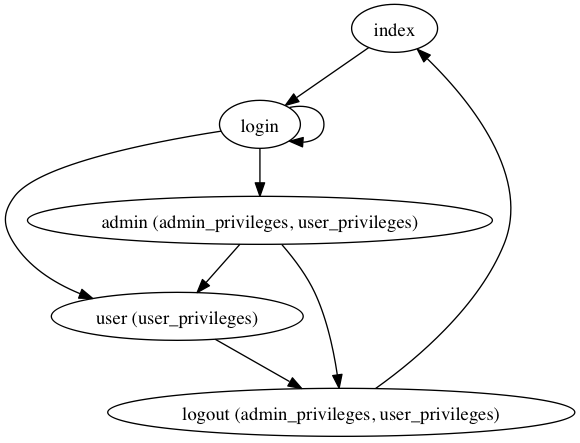
\includegraphics[scale=0.5]{model.png}
\caption{En webbsida med användarhantering.}
\end{figure}

\begin{figure}
\lstinputlisting[language=Prolog]{../src/lab2.pl}
\end{figure}

\end{document}
